\documentclass[12pt, class=report, crop=false]{standalone}
\usepackage{ba_thesis}

\begin{document}

\chapter{Results}%
\label{chap:results}

This chapter covers the results from the numerical simulations that I've run using the EPOCH Particle-in-Cell code. The main focus of the study is to analyze the use of Laguerre-Gauss modes in laser wakefield accelerators and to compare their behaviour with that of simple Gaussian modes. The simulations were performed using the computing cluster from the Departament of Computational Physics and Information Technology of the National Institute of Phisics and Nuclear Engineering. The servers used had an Intel\textsuperscript{\tiny\textregistered} Xeon\textsuperscript{\tiny\textregistered} E 5-2640 v4 2.4 GHz (3.4 GHz Turbo Boost) processor. Each server has 10 cores per socket and 128 GB RAM memory. MPI was used for parallelization, and benchmarks showed that running with Hyper-Threading or running on two servers at once improves the computation time significantly. For all simulations I chose the latter option, the average simulation time being somewhere between half a day and a full day (the duration is so long because all the simulations were 3D).

\section{Low intensity laser simulations}

The fisrt set of simulations was done with low intensity \(1\; \mu\)m wavelength lasers, namely \(a_0 = 2\), or, equivalently, \(I = 5.65 \cp 10^{18}\) W/cm$^2$. Also, \(w_0 = 5\lambda\) was chosen. The domain size was 60$\lambda$ $\cp$ 30$\lambda$ $\cp$ 30$\lambda$, discretized with a grid of 1200 $\cp$ 300 $\cp$ 300. Notice that the grid is much finer on the x direction (in our simulations this is the propagation direction) than in the y and z directions. This is done in order to reduce the compilation time, since the main physical effects as well as the structures we want to observe are along the propagation direction of the laser. There are three such simulations, one with the Gauss beam, and two with the (m = 1, p = 0) and (m = 2, p = 0) Laguerre-Gauss beams. An example of input.deck file with comments about how the different profiles are implemented is given in the Appendix.

With this first set of simulations we are interested to see if coherent beams of accelerated electrons are formed and to compare the acceleration efficiency across the different laser profiles used. For the second purpose, the energy density (the product between the average energy per particle and the particle number density, computed locally at each point on the grid) of the electrons was found to be a relevant quantity. This is because, in the region of the accelerated beam, both the average electron energy and the electron number density are high compared with the rest of the electrons in the medium. As such, this energy density has visible spikes at the location of the electron beam. We can also use the maximum of this quantity at each time step to follow the acceleration process and its efficiency (while the exact values are to be taken with a grain of salt, we can extract information from trends and orders of magnitude). It is known that in the process of acceleration in LWFA, there is first an increase in the electron beam energy and then a decrease. As such, this method is efficient over a certain region, and knowing the limits of that region is important when designing the actual accelerators. This pattern of variation is also observed in the maximum values of the electron energy density taken at each step. In the following figures, details related to this and other aspects are illustrated. All figures have the corner facing the reader clipped in order to see inside the structures formed (the structures are highly symmetrical).

\begin{figure}[!h]
  \centering
  \includegraphics[width=1.0\textwidth]{/thesis-pics/sim-1.0/visit0000}%
  \caption{A pseudocolor plot cut with isosurfaces of the electron energy density that shows more levels for low values. This is done in order to observe the plasma wave electrons, such that the beam, as well as the bubble shape and the laser position can be seen clearly. We see that since the intensity is low, the bubble is not depleted completely, and we can clearly see the electrons interacting with the laser. At high intensity, the ponderomotive force is much larger and the electrons are pushed outside the laser region very fast, so the bubble is depleted of electrons.}
  \label{fig:visit0000}%
\end{figure}

\begin{figure}[!h]
  \centering
  \begin{subfigure}[t]{0.47\textwidth}
    \centering
    \includegraphics[width=1.0\textwidth]{/thesis-pics/sim-1.0/visit0001}
  \end{subfigure}
  \hfill
  \begin{subfigure}[t]{0.47\textwidth}
    \centering
    \includegraphics[width=1.0\textwidth]{/thesis-pics/sim-1.0/visit0003}
  \end{subfigure}
  \vskip\baselineskip
  \begin{subfigure}[b]{0.47\textwidth}
    \centering
    \includegraphics[width=1.0\textwidth]{/thesis-pics/sim-1.0/visit0005}
  \end{subfigure}
  \hfill
  \begin{subfigure}[b]{0.47\textwidth}
    \centering
    \includegraphics[width=1.0\textwidth]{/thesis-pics/sim-1.0/visit0007}
  \end{subfigure}
  \caption{A series of pseudocolor plots of the electron energy density using isosurfaces showing the electron beam at different moments in time: 200 fs (top-right), 250 fs (top-left), 300 fs (bottom-right), 350 (bottom-left). }%
  \label{fig:beam-gauss}%
\end{figure}

\begin{figure}[!h]
  \centering
  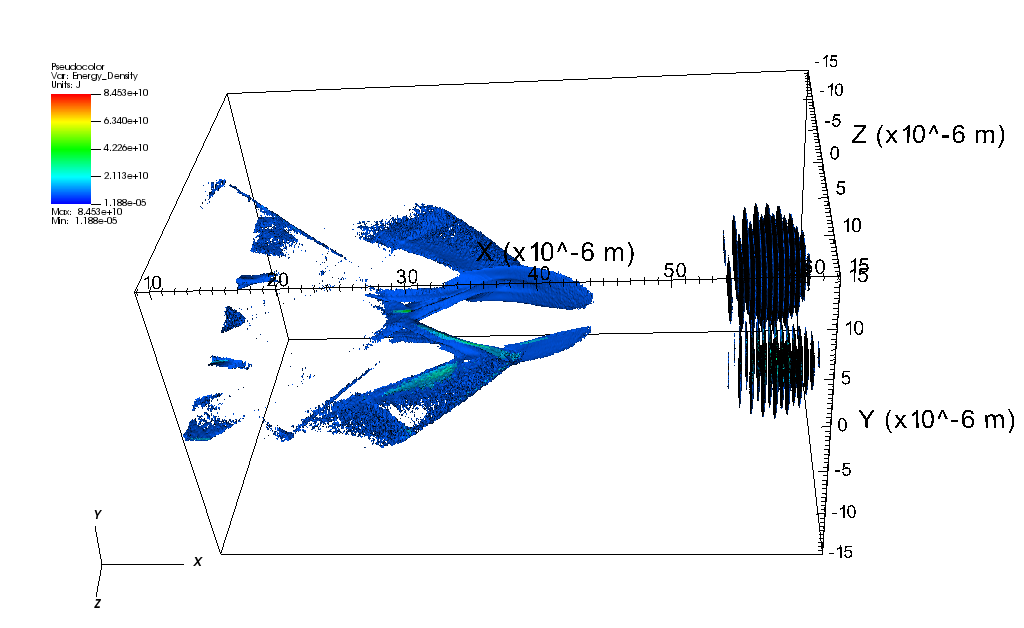
\includegraphics[width=1.0\textwidth]{/thesis-pics/sim-1.0/visit0012}%
  \caption{A pseudocolor plot cut with isosurfaces (10) of the electron energy density for the m=1, p=0 Laguerre-Gauss mode (330 fs).}
  \label{fig:visit0012}%
\end{figure}

\begin{figure}[!h]
  \centering
  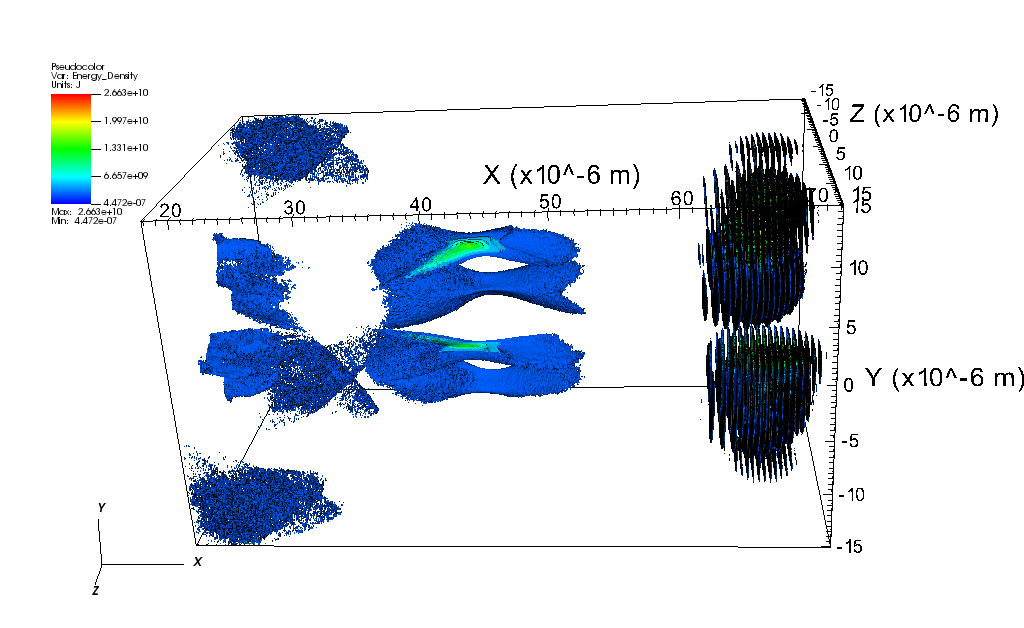
\includegraphics[width=0.95\textwidth]{/thesis-pics/sim-1.0/visit0013}%
  \caption{A pseudocolor plot cut with isosurfaces (10) of the electron energy density for the m=2, p=0 Laguerre-Gauss mode (360 fs).}
  \label{fig:visit0013}%
\end{figure}

\begin{figure}[!h]
  \centering
  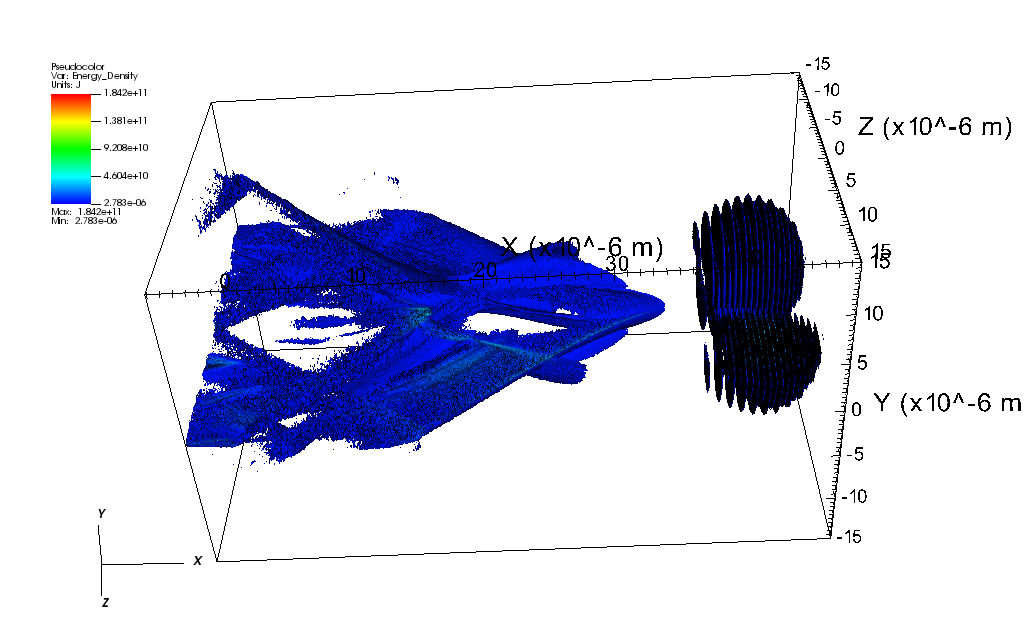
\includegraphics[width=0.95\textwidth]{/thesis-pics/sim-1.0/visit0011}%
  \caption{A pseudocolor plot cut with isosurfaces (50) of the electron energy density for the m=1, p=0 Laguerre-Gauss mode (280 fs). We made a large number of isosurfaces to see the much more complicated patters of the low energy electrons compared to the very simple one in the case of the regular Gauss profile.}
  \label{fig:visit0011}%
\end{figure}

\begin{figure}[!h]
  \centering
  \includegraphics[width=0.95\textwidth]{/thesis-pics/visit0000}%
  \caption{A pseudocolor plot cut with isosurfaces of the magnitude of the electric field vector at each of the grid points in the case of the simple Gaussian profile. This plot indicates the shape of the profile.}
  \label{fig:laserbeam-gauss}%
\end{figure}

\begin{figure}[!h]
  \centering
  \begin{subfigure}[t]{0.6\textwidth}
    \centering
    \includegraphics[width=1.0\textwidth]{/epoch-simulation-results/laser-wakefield-laguerre/m1p0/visit0000}
  \end{subfigure}
  \hfill
  \begin{subfigure}[t]{0.6\textwidth}
    \centering
    \includegraphics[width=1.0\textwidth]{/epoch-simulation-results/laser-wakefield-laguerre/m2p0/visit0000}
  \end{subfigure}
  \caption{A series of pseudocolor plots cut with isosurfaces of the magnitude of the electric field vector at each of the grid points in the case of the m=1, p=0 (top) and the m=2, p=0 Laguerre-Gauss profiles. This plot indicates the shape of the profiles.}%
  \label{fig:laserbeam-laguerre}%
\end{figure}

\begin{figure}[!h]
  \centering
  \begin{subfigure}[t]{0.85\textwidth}
    \centering
    \includegraphics[width=1.0\textwidth]{/thesis-pics/Ponderomotive-Force/visit0000}
  \end{subfigure}
  \hfill
  \begin{subfigure}[t]{0.85\textwidth}
    \centering
    \includegraphics[width=1.0\textwidth]{/thesis-pics/Ponderomotive-Force/visit0001}
  \end{subfigure}
  \caption{Vector plots showing the ponderomotive force for the m=1 Laguerre profile from different angles.}
  \label{fig:ponderomotive-force-1}%
\end{figure}

\begin{figure}[!h]
  \centering
  \begin{subfigure}[t]{0.85\textwidth}
    \centering
    \includegraphics[width=1.0\textwidth]{/thesis-pics/Ponderomotive-Force/visit0002}
  \end{subfigure}
  \hfill
  \begin{subfigure}[t]{0.85\textwidth}
    \centering
    \includegraphics[width=1.0\textwidth]{/thesis-pics/Ponderomotive-Force/visit0003}
  \end{subfigure}
  \caption{Vector plots showing the ponderomotive force for the m=2 Laguerre profile from different angles.}
  \label{fig:ponderomotive-force-2}%
\end{figure}

As shown in~\cref{fig:visit0000}, there is a singular clear coherent beam of accelerated electrons. Close-ups on the beam are shown in~\cref{fig:beam-gauss}. In contrast,~\cref{fig:visit0011} reveals that the plasma wave generated by the passing of the laser through the plasma is much more complicated for the Laguerre modes. There is no longer a clear bubble-beam-bubble pattern visible, and as such we can see no longer a clear electron beam forming on the propagation axis. However,~\cref{fig:visit0012,fig:visit0013} shed light on this matter. It seems that there are electron beams forming, but there are two of them for m=1 and four of them for m=4. We connect this occurance with the topology of the profiles. It is clear what we mean by this if we first take a look at~\cref{fig:laserbeam-gauss,fig:laserbeam-laguerre}. We can see that the plots of the magnitude of the electric field (which reflect the geometrical shape of each profile, since the field of the particles is screened by plasma mechanisms) show one connected structure in the case of the Gauss beam, but in the case of the Laguerre profiles there are disjointed structures. The number of disjointed structures is equal to the number of electron beams forming and is also equal to 2m. This, together with the visual hints in~\cref{fig:visit0012,fig:visit0013} (the electron beams are formed behind each structure) suggest that the independent effect of each structure is not strongly influenced the other structures, so each of them acts like a Gauss beam on its own.

\begin{table}[!h]
\begin{tabular}{|c|c|c|c|c|c|}
\hline
\multicolumn{6}{|c|}{Maximum Value of Electron Energy Density} \\ \hline
\multicolumn{2}{|c|}{\begin{tabular}[c]{@{}c@{}}Gauss\\ m=0\end{tabular}} & \multicolumn{2}{|c|}{\begin{tabular}[c]{@{}c@{}}Laguerre\\ m=1\end{tabular}} & \multicolumn{2}{|c|}{\begin{tabular}[c]{@{}c@{}}Laguerre\\ m=2\end{tabular}} \\ \hline
\begin{tabular}[c]{@{}c@{}}Enrgy Value\\ ($10^{10}$ J/m\textsuperscript{3})\end{tabular} & \begin{tabular}[c]{@{}c@{}}Simulation Time\\ (fs)\end{tabular} & \begin{tabular}[c]{@{}c@{}}Enrgy Value\\ ($10^{10}$ J/m\textsuperscript{3})\end{tabular} & \begin{tabular}[c]{@{}c@{}}Simulation Time\\ (fs)\end{tabular} & \begin{tabular}[c]{@{}c@{}}Enrgy Value\\ ($10^{10}$ J/m\textsuperscript{3})\end{tabular} & \begin{tabular}[c]{@{}c@{}}Simulation Time\\ (fs)\end{tabular} \\ \hline
652.8 & 200 & 34.3 & 180 &11 & 160 \\ \hline
584.1 & 250 & 28.1 & 230 & 9.9 & 210 \\ \hline
420.1 & 300 & 18.4 & 280 & 6.2 & 260 \\ \hline
366.5 & 350 & 8.4  & 330 & 8.8 & 310 \\ \hline
500.6 & 400 & 4.7  & 380 & 2.66 & 360 \\ \hline
\end{tabular}
\caption{A table with the maximum value of electron energy density at different time steps. The first value for each profile was taken to be the overall maximum in the simulation, which corresponds to the moment of time in which the acceleration has peaked. After that, values are taken in intervals of 50 fs. The data reflects the post acceleration energy loss part of the LWFA process.}
\label{table:1}
\end{table}

One possible physical explanation for this effect would be related to the intensity of the lasers. Since the intensity is quite low, so is the ponderomotive force. Because of this, there are still electrons remaining in the laser region, which oscillate in the laser's fields until it gets out, and are almost equally probable to leave through the outside as well through the in between region. We say almost because in~\cref{fig:ponderomotive-force-1,fig:ponderomotive-force-2} we can see a small ponderomotive force component towards the center region. These electrons could leave through the space in between the lumps of the Laguerre beams, as visible in~\cref{fig:visit0011}. Also, there is no  ponderomotive force in the space between the structures as shown in~\cref{fig:ponderomotive-force-1,fig:ponderomotive-force-2}, so thermal electrons passing through there don't interact strongly with the laser. This effect is expected to dissapear at higher intensities, since the laser region is expected to be depleted of electrons extremely fast. Nonetheless, the effect in itself could posses practical application. This study suggests that for intensities of the order of $10^{18}$ W/cm$^2$, by utilizing Laguerre-Gauss modes, it is possible to obtain multipe beams of accelerated electrons arranged in well defined patterns. In~\cref{table:1}, we show values of the electron energy density in order to compare the acceleration efficiency across different profiles. By analizing the data, we saw that the maximum value of this quantity follows the pattern of acceleration followed by slow down characteristic to LWFA. The values in the table start with the overall maximum (the peak of acceleration) and follow the energy loss in time after that. We can see that by increasing m with one unit at a time we see a loss of energy density in the beams of about one order of magnitude. So, there is a trade off between the number of beams achieved in this manner and the efficacity of the accelerator. This supports the theory that each of the structures in the Laguerre beams acts as an almost independent weaker Gaussian beam at low intensities.

\section{Higher intensity laser simulations}

In the second set of simulations, we aimed to have laser intensities of the order of $10^{22}$ W/cm$^2$. In order to do this, changes in the simulations parameters have to be made (The laser shape spreads transversally with increases in electric field amplitude, so the comain size must be changed, which in turn requires the reevaluation of the grid discretization). We settled for a \(\lambda = 0.8\) \(\mu\)m, \(a_0=70\), and \(w_0 = 7\lambda\) laser (\(I = 1.082\cp 10^{22}\) W/cm$^2$). The domain was taken to be 100\(\lambda\) $\cp$ 50\(\lambda\) $\cp$ 50\(\lambda\), with a grid of 1000 $\cp$ 250 $\cp$ 250. This time around we only look at the regular Gauss profile and the first Laguerre mode (m=1). We aim again to compare the effects of the two profiles and see the differences that arise with the increase in intensity. The methods used for analysis are similar to those in the previous section. The input.deck file for the EPOCH simulation is also made available in the Appendix.

In~\cref{fig:density-sim-2} we show the density of electrons for the two simulations in order to visualize the plasma wave pattern formed. We can clearly see the formation of beams as well as the bubbles in front and behind it. This time, the bubble is clearly depleted. We can see also that the pattern repeats itself, there being a secondary bunch of electrons behind the second bubble and so on. This is a well known occurance. However, only the first bunch of electrons is well accelerated, being both dense and energetic. This time around, the Laguerre-Gauss mode also forms one coherent accelerated beam of electrons instead of multiple ones. This is also visible in~\cref{fig:beams-sim-2}, where we look at the energy density to see better the shape and structure of the electron bunches. We can see that the Laguerre generated beam has a kind of doughnut shape, compared to the Gauss generated one, which has more flat transversal sections. In order to understand better the difference in shapes, we indicate~\cref{fig:laserbeams-sim-2,fig:laserbeams2-sim-2}. They show the electric field magnitude in two manners, illustrating the shape of the laser profiles. We can again see the separation of two clear structures in the Laguerre-Gauss beam, which this time around is not large enough to make the structures act independently, but causes the doughnut shape of the electron beam. The disturbances seen at the tail of the laser bumps are in the electron bunch region, and reflect the electric fields generated by high densities of electrons. We also plotted the ponderomotive force for the Laguerre mode~\cref{fig:ponderomotive-force-3} for visual comparison with the previous simulation.

\begin{table}[!h]
\centering
\begin{tabular}{c|c|l|c|l|l|l|}
\cline{2-7}
\multicolumn{1}{l|}{} & \multicolumn{6}{c|}{Maximum Value of Electron Energy Density} \\ \cline{2-7}
\multicolumn{1}{l|}{} & \multicolumn{2}{c|}{\begin{tabular}[c]{@{}c@{}}Gauss\\ m=0\end{tabular}} & \multicolumn{4}{c|}{\begin{tabular}[c]{@{}c@{}}Laguerre\\ m=1\end{tabular}}\\ \hline
\multicolumn{1}{|c|}{\begin{tabular}[c]{@{}c@{}}Simulation Time\\ (fs)\end{tabular}} & \multicolumn{2}{c|}{\begin{tabular}[c]{@{}c@{}}Enrgy Value\\ ($10^{18}$ J/m$^3$)\end{tabular}} & \multicolumn{4}{c|}{\begin{tabular}[c]{@{}c@{}}Enrgy Value\\ ($10^{18}$ J/m$^3$)\end{tabular}} \\ \hline
\multicolumn{1}{|c|}{150}  & \multicolumn{2}{c|}{1.47}  & \multicolumn{4}{c|}{1.59}  \\ \hline
\multicolumn{1}{|c|}{180}  & \multicolumn{2}{c|}{2.67}  & \multicolumn{4}{c|}{3.04}  \\ \hline
\multicolumn{1}{|c|}{210}  & \multicolumn{2}{c|}{2.65}  & \multicolumn{4}{c|}{2.35}  \\ \hline
\multicolumn{1}{|c|}{240}  & \multicolumn{2}{c|}{3.68}  & \multicolumn{4}{c|}{2.05}  \\ \hline
\multicolumn{1}{|c|}{270}  & \multicolumn{2}{c|}{3.53}  & \multicolumn{4}{c|}{1.83}  \\ \hline
\multicolumn{1}{|c|}{300}  & \multicolumn{2}{c|}{2.70}  & \multicolumn{4}{c|}{2.00}  \\ \hline
\end{tabular}
\label{table:2}
\caption{A table with the maximum value of electron energy density at different time steps.}
\end{table}

Finally, we again compare the values of electron energy density to compare acceleration efficiency. Due to the changes in initial parametes and the reduction in the simulation duration (for run time reduction), we can not see the entirety of the two acceleration for bots profiles, but we cath the region around the peak for both. We therefore show in~\cref{table:2} simultaneous values. The main observation is that this time around the order of magnitude is the same, which suggest the by using Laguerre-Gauss modes at high intensities should not affect the acceleration efficiency substantially.

\begin{figure}[!h]
  \centering
  \begin{subfigure}[t]{1\textwidth}
    \centering
    \includegraphics[width=1.0\textwidth]{/thesis-pics/sim-1.1/visit0001}
  \end{subfigure}
  \hfill
  \begin{subfigure}[t]{1\textwidth}
    \centering
    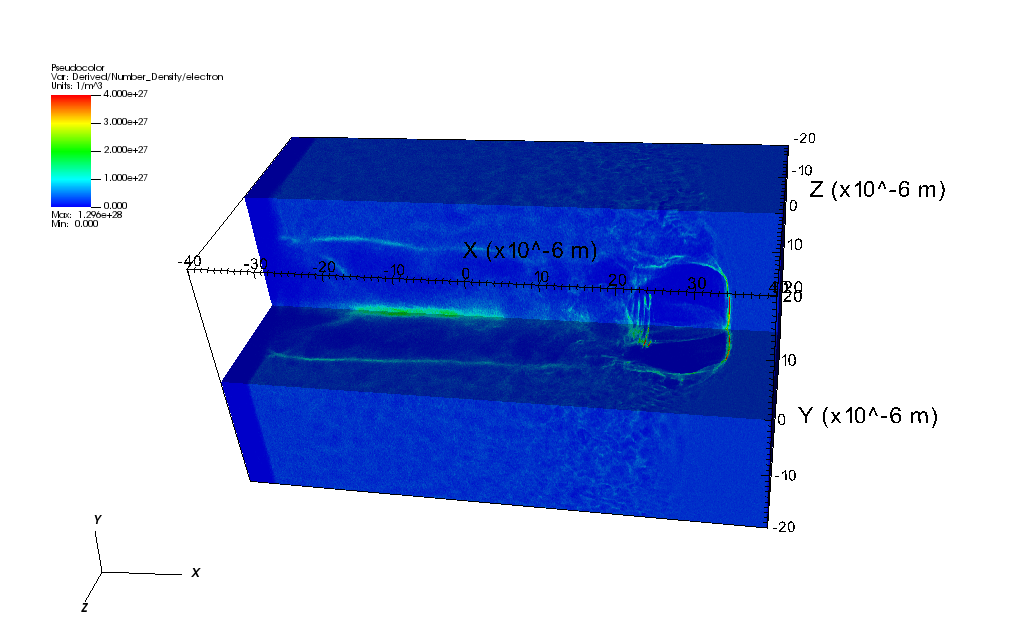
\includegraphics[width=1.0\textwidth]{/thesis-pics/sim-1.1/visit0008}
  \end{subfigure}
  \caption{Plots of the number density of electrons across the entire simulation domain at 255 fs into the run: top - Gauss, Bottom - Laguerre. The upper limit of the color bar was set below the actual maximum value in the data in order to emphasize the low density fluctuations for visual clarity.}%
  \label{fig:density-sim-2}%
\end{figure}

\begin{figure}[!h]
  \centering
  \begin{subfigure}[t]{1\textwidth}
    \centering
    \includegraphics[width=1.0\textwidth]{/thesis-pics/sim-1.1/visit0004}
  \end{subfigure}
  \hfill
  \begin{subfigure}[t]{1\textwidth}
    \centering
    \includegraphics[width=1.0\textwidth]{/thesis-pics/sim-1.1/visit0005}
  \end{subfigure}
  \caption{Pseudocolor plots of isosurfaces of the electron energy density at 270 fs into the run: top - Gauss, Bottom - Laguerre.}%
  \label{fig:beams-sim-2}%
\end{figure}

\begin{figure}[!h]
  \centering
  \begin{subfigure}[t]{1\textwidth}
    \centering
    \includegraphics[width=1.0\textwidth]{/thesis-pics/sim-1.1/visit0000}
  \end{subfigure}
  \hfill
  \begin{subfigure}[t]{1\textwidth}
    \centering
    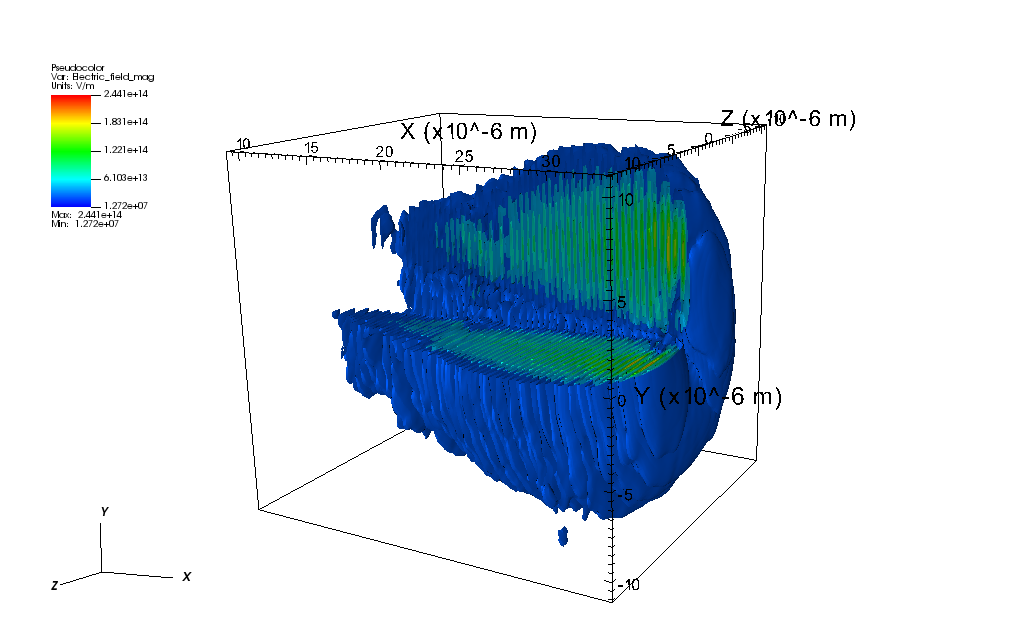
\includegraphics[width=1.0\textwidth]{/thesis-pics/sim-1.1/visit0006}
  \end{subfigure}
  \caption{Plots of isosurfaces of the the electric field magnitude: top - Gauss, Bottom - Laguerre.}%
  \label{fig:laserbeams-sim-2}%
\end{figure}

\begin{figure}[!h]
  \centering
  \begin{subfigure}[t]{1\textwidth}
    \centering
    \includegraphics[width=1.0\textwidth]{/thesis-pics/sim-1.1/visit0002}
  \end{subfigure}
  \hfill
  \begin{subfigure}[t]{1\textwidth}
    \centering
    \includegraphics[width=1.0\textwidth]{/thesis-pics/sim-1.1/visit0007}
  \end{subfigure}
  \caption{Plots of the the electric field magnitude in the volume: top - Gauss, Bottom - Laguerre.}%
  \label{fig:laserbeams2-sim-2}%
\end{figure}

\begin{figure}[!h]
  \centering
  \begin{subfigure}[t]{0.85\textwidth}
    \centering
    \includegraphics[width=1.0\textwidth]{/thesis-pics/Ponderomotive-Force/visit0004}
  \end{subfigure}
  \hfill
  \begin{subfigure}[t]{0.85\textwidth}
    \centering
    \includegraphics[width=1.0\textwidth]{/thesis-pics/Ponderomotive-Force/visit0005}
  \end{subfigure}
  \caption{Vector plots showing the ponderomotive force for the m=1 Laguerre profile from different angles.}
  \label{fig:ponderomotive-force-3}%
\end{figure}

\section{Stuctured targets}

This study surrounds certain aspects of the production of gamma
-beams using the interaction between a laser pulse and a plasma medium
with a predesigned structure. To be more specific, we simulate the
passage of a simple Gaussian pulse through a pipe-like overdense
carbon plasma structure using a Particle-in-Cell code (EPOCH). The
plasma pipe consists of a cylindrical bulk region, with the density
100 \(n_{crit}\), surrounding a cylindrical channel, with the density
20 \(n_{crit}\) (see~\cref{fig:pipe}). The channel diameter is
comparable with the laser beam waist radius, such that most of the
energy transferred from it to the plasma goes into the channel region. The
propagation of the laser through the channel drives a longitudinal
electron current (see~\cref{fig:electron-current}), which in turn
generates and sustains a quasistatic azimuthal magnetic field. By
deflecting the highly energetic electrons, this field induces the
production of synchrotron photons. The result is a gamma-beam with a
relatively small divergence. For more details related to this see the article by~\cite{wangPowerScalingCollimated2020}, which is the one that lead us to doing this study. This type of technique has the advantage of being easier to implement experimentally than the change in laser profile used in the previous two sections.

\begin{figure}[!h]
  \centering
  \includegraphics[width=1.0\textwidth]{/thesis-pics/structured-target/1PW/visit0000}%
  \caption{A plot of the electron number density at the beginning of
  the simulation showcasing the structure of the carbon plasma used
  for the numerical experiments.}
  \label{fig:pipe}%
\end{figure}

We aim to study the variation of the gamma yield
with the change in the internal radius of the pipe
(\textit{i}.\textit{e}. the channel radius), while keeping the
external radius fixed. For the parametrization of the laser we chose
the defining parameters to be: \(a_0 = 190\), \(\lambda_0 = 1\)
\(\mu\)m, which lead to a peak intensity of \(5\cp10^{22}\) W/
cm\(^{2}\). We remark that this value of laser peak intensity is in
general relevant for the new Petawatt laser infrastructures around
the world. We also chose the beam waist radius to be \(w_0 = 1.3\)
\(\mu\)m, which sets the power of our laser to 1 PW. The laser was
focalized at \(x = 0.0\) and the pulse duration was 35 fs. The
exterior radius of the pipe was fixed to 4 \(\mu\)m, while the
interior radius was given the values: \(0.5w_0\), \(0.7w_0\),
\(1.0w_0\), and \(1.2w_0\). The total length of the pipe was set to
33 \(\mu\)m and the total simulation time was chosen to be 110 fs.
In all simulations the plasma was initiallized as being fully
ionized, since studies in the literature suggest that at the
intensity and the power we work with the initially neutral medium
would become fully ionized almost instantly. For the grid,
we used a distretization of 30/\(\mu\)m in all three spatial
directions. Since we are only interested to look
at the energy of the produced photons, we have set them in the
simulation to not propagate in time (that is, after they are
produced, they are registered and not used further in the simulation),
thus reducing greatly the simulation time. The average simulation time
was 26 hours. An example input.deck is again available in the Appendix, this time together with a short indication on how to enable the QED effects in EPOCH.

\begin{figure}[!h]
  \centering
  \includegraphics[width=1.0\textwidth]{/thesis-pics/structured-target/1PW/visit0002}%
  \caption{A plot of the electron energy density (average electron energy multiplied by the number density) that showcases the electron current generated in the channel.}
  \label{fig:electron-current}%
\end{figure}

In~\cref{fig:photons} we show the energy distribution in volume of the photon energy for the photons generated up to 100 fs into the simulation. By analyzing the data, we find that photons are generated, as expected, predominantly inside the channel region. From the transversal section we can observe better the internal structure of the photon bulk. We can clearly see that it hints towards the spherical projections given in~\cref{wangPowerScalingCollimated2020} on page 3.

\begin{figure}[!h]
  \centering
  \begin{subfigure}[t]{0.47\textwidth}
    \centering
    \includegraphics[width=1.0\textwidth]{/thesis-pics/structured-target/photons/visit0000}
  \end{subfigure}
  \hfill
  \begin{subfigure}[t]{0.47\textwidth}
    \centering
    \includegraphics[width=1.0\textwidth]{/thesis-pics/structured-target/photons/visit0001}
  \end{subfigure}
  \vskip\baselineskip
  \begin{subfigure}[b]{0.47\textwidth}
    \centering
    \includegraphics[width=1.0\textwidth]{/thesis-pics/structured-target/photons/visit0002}
  \end{subfigure}
  \hfill
  \begin{subfigure}[b]{0.47\textwidth}
    \centering
    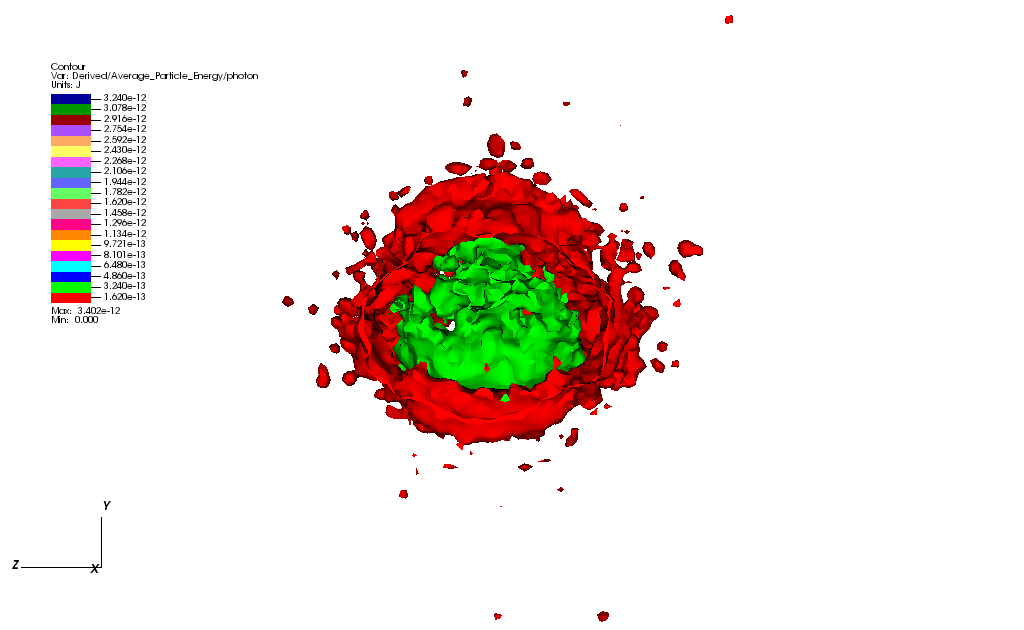
\includegraphics[width=1.0\textwidth]{/thesis-pics/structured-target/photons/1microns_in}
  \end{subfigure}
  \vskip\baselineskip
  \begin{subfigure}[b]{0.47\textwidth}
    \centering
    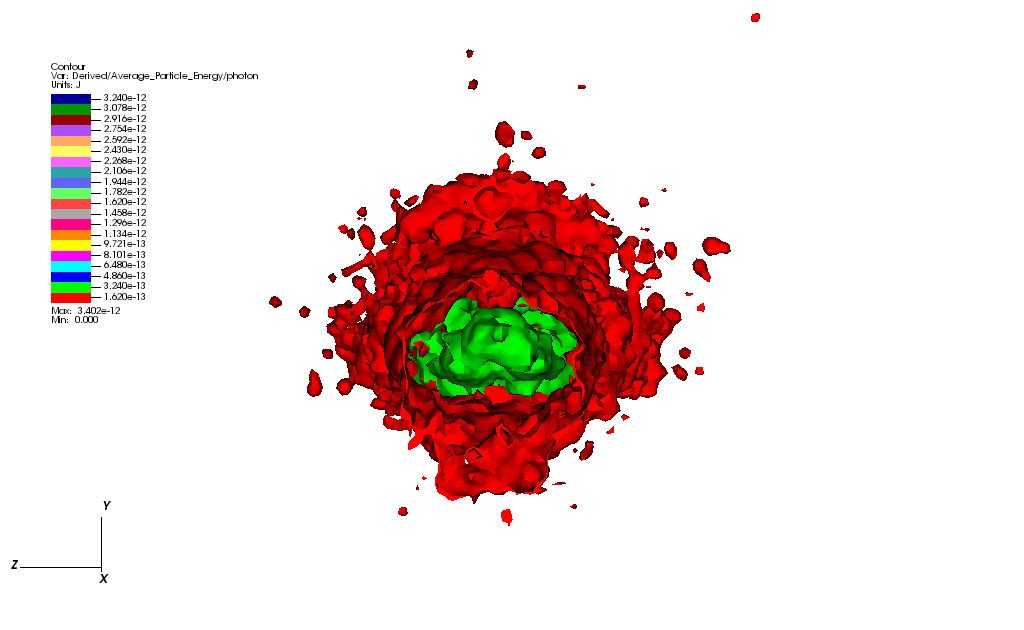
\includegraphics[width=1.0\textwidth]{/thesis-pics/structured-target/photons/3microns_in}
  \end{subfigure}
  \hfill
  \begin{subfigure}[b]{0.47\textwidth}
    \centering
    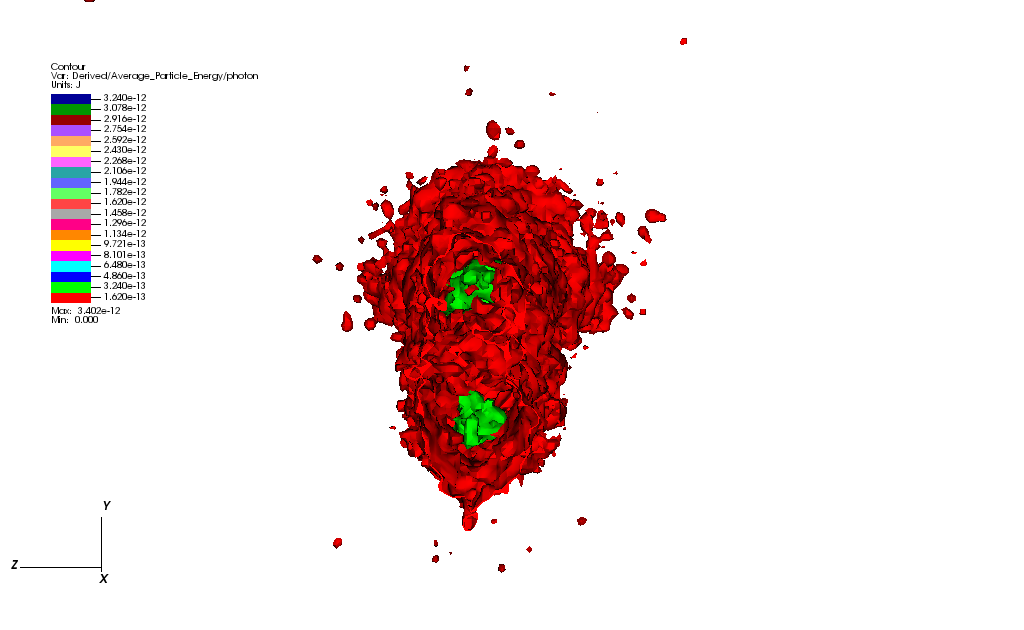
\includegraphics[width=1.0\textwidth]{/thesis-pics/structured-target/photons/6microns_in}
  \end{subfigure}
  \caption{A series of contour plots of the average photon energy showcasing all the photons produced up to 100fs into the simulation. Different plots show different clips of the photon bulk. They are displayed in the following order: top left - uncut view; top right - cut through the middle in the x-z plane; middle left - cut through the middle in the x-y plane; middle right - transversal cut 1 \(\mu\)m in from the entry plane of the laser; bottom left - - transversal cut 3 \(\mu\)m in from the entry plane of the laser; bottom right - transversal cut 6 \(\mu\)m in from the entry plane of the laser.}%
  \label{fig:photons}%
\end{figure}

\begin{figure}[!h]
  \centering
  \includegraphics[width=1.0\textwidth]{/thesis-pics/structured-target/1PW/visit0001}%
  \caption{A plot of the electron number density 100 fs into the simulation that showcases how the passage of the laser through the plasma affects the sructure of our plasma pipe. Some channel electrons spread inside the bulk region.}
  \label{fig:electron-current}%
\end{figure}

In order to compare the photon production as a function of channel radius, we look at the average particle energy per grid cell. We count all the cells that contain an average energy larger than a certain lower limit. The results are shown in~\cref{fig:efficiency}. In this plot, by efficiency we actually mean the number of grid cell with average energy above a ceratain value divided by the total number of grid cells that contain non-zero values of photon energy. This is used as a way to estimate the fraction of photons above certain energies from the total number of photons produced in the simulation. We can see that both graphs show an increase with the increase of the channel radius. This trend is more pronounced in the low energy samples. We also note that the cuves are concave, which suggests that further increase of the channel radius will not continue to increase the synchrotron photon yield. This is expected, since further increase in the radius would make the channel much thicker than the laser beam.

\begin{figure}[!h]
  \centering
  \begin{subfigure}[t]{0.9\textwidth}
    \centering
    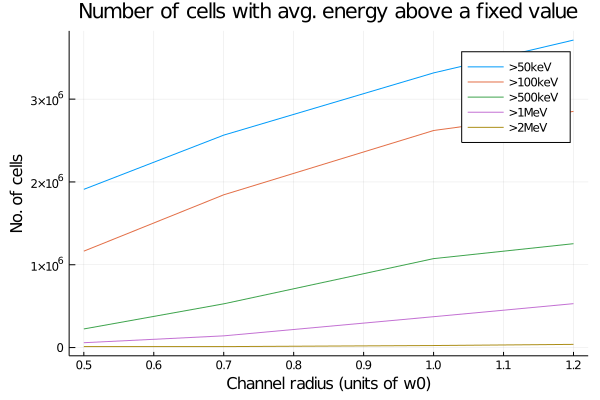
\includegraphics[width=1.0\textwidth]{/thesis-pics/structured-target/energies}
  \end{subfigure}
  \hfill
  \begin{subfigure}[t]{0.9\textwidth}
    \centering
    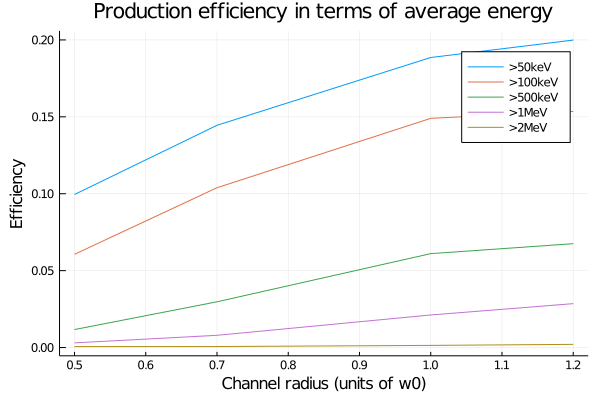
\includegraphics[width=1.0\textwidth]{/thesis-pics/structured-target/efficiency}
  \end{subfigure}
  \caption{Plots comparing the production yield of different photon energies in terms of the channel radius. Top: the number of cells with average photon energy above 50 keV, 100 keV, 500 keV, 1 Mev, and 2 MeV, respectively. Bottom: the production efficiency for different energies above the same lower limits as in the previous plot.}%
  \label{fig:efficiency}%
\end{figure}

\end{document}
